\chapter{Teori Probabilitas}
\section{Pendahuluan}
Teori probabilitas digunakan untuk mengkuantifikasikan ketidakpastian. Teori probabilitas menyediakan aksioma - aksioma yang dapat digunakan untuk menurunkan pernyataaan - pernyataan matematis tentang ketidakpastian.

Di bidang analisis data sendiri, hukum - hukum probabilitas digunakan sebagai fondasi tentang bagaimana suatu sistem algoritma menimbang permasalahan dan memberikan keputusan untuk menyelesaikan permasalahan tersebut. Dapat dikatakan bahwa teori probabilitas merupakan batu penjuru dari kemampuan dari suatu sistem kecerdasan buatan untuk dapat berpikir dan menimbang permasalahan selayaknya manusia biasa yang kesehariannya tidak luput dari ketidakpastian.

Terdapat tiga macam sumber ketidakpastian ketika kita hendak menganalisis data, yakni:
\begin{itemize}
	\item Ketidakpastian stokastik yang bersifat inheren, yakni secara natural sistem yang hendak kita modelkan diatur oleh hukum - hukum alam yang bersifat tidak pasti. Contoh yang paling terkenal adalah pemodelan mekanika kuantum.
	\item Ketidaklengkapan hasil observasi. Dalam kasus ini kita tidak mempunyai seluruh data yang hendak dimodelkan. Jenis ketidakpastian inilah yang utamanya sering dijumpai ketika kita melakukan penganalisisan data. Misalnya, ketika kita hendak menerapkan algoritma pengenalan objek - objek lalulintas pada mobil swakemudi, tentu kita hanya melatih sistem tersebut dengan ratusan (atau bahkan ribuan) objek - objek fotografi rambu - rambu lalulintas, sedangkan pada kenyataannya mobil swakemudi ini harus berhadapan dengan seluruh rambu - rambu lalulintas di seluruh jalan raya di Indonesia.
	\item Ketidaklengkapan pemodelan. Seringkali karena keterbatasan sumberdaya komputasi kita hanya memodelkan beberapa fitur penting saja, sehingga beberapa fitur yang mendetail sengaja kita abaikan karena keterbatasan sumberdaya komputasi. Salah satu contohnya adalah pemodelan iklim global yang mungkin saja gagal menangkap fenomena regional seperti sistem monsun.
\end{itemize} 

Oleh karena tiga ketidakpastian tersebut, kita membutuhkan teori probabilitas untuk memodelkan data yang telah kita peroleh. 

Berdasarkan kesepakatan para ilmuwan, teori probabilitas terbagi ke dalam dua mazhab utama, yakni:
\begin{itemize}
	\item Probabilitas frekuensi, yang mana lebih menekankan pada frekuensi terjadinya suatu kejadian tertentu. Contohnya adalah seberapa sering kita memperoleh dadu dengan jumlah enam ketika dua kali melemparkan dadu.
	\item Probabilitas Bayesian, yang mana lebih menekankan pada derajat kepercayaan. Contohnya adalah ketika dokter menyatakan seorang pasien mempunyai 40\% peluang terjangkit COVID-19.
\end{itemize}
\section{Distribusi - distribusi probabilitas}
\subsection{Peubah acak}
Peubah acak (\textit{random variable}) merupakan suatu peubah yang dapat memperoleh nilai secara acak dari suatu himpunan nilai. Peubah acak $X$ dapat memperoleh nilai dari himpunan bilangan $\{x_{1}, x_{2}, x_{3}, \cdots, x_{n}\}$. Distribusi probabilitas sendiri bertugas untuk menentukan seberapa besar peluang suatu nilai di dalam himpunan bilangan yang dimaksud untuk terpilih sebagai peubah acak. Terdapat dua jenis peubah acak, yakni:
\begin{itemize}
\item \textbf{Diskrit}, yang mana mempunyai nilai - nilai tertentu (bersifat finit), dan
\item \textbf{Kontinyu}, yang mana himpunan kandidat peubah acak tersebut merupakan bilangan riil yang bersifat kontinyu.
\end{itemize} 

\subsection{Fungsi massa peluang} 
Distribusi probabilitas untuk peubah acak diskrit dikenal sebagai fungsi massa peluang (\textit{Probability Mass Function}: PMF). Terdapat tiga kriteria yang menyatakan bahwa suatu fungsi dapat dikategorikan sebagai PMF:
\begin{itemize}
\item Domain dari $P$ harus memenuhi setiap nilai dari $x$.
\item $0 \leq P(X) \leq 1$
\item $\Sigma P(X) = 1$, oleh karena itu distribusi probabilitas pada PMF selalu ternormalisasi.
\end{itemize}

Terdapat dua jenis PMF, yakni:
\begin{itemize}
	\item Distribusi probabilitas gabungan, yang mana merupakan PMF yang berlaku pada banyak peubah. $P(X=x, Y=y)$ berlaku untuk setiap $X=x$ dan $Y=y$ secara bersamaan.
	\item  Distribusi seragam, pada distribusi ini seluruh elemen di dalam himpunan peubah acak mempunyai peluang yang sama untuk terpilih. Berikut adalah formulasi umumnya (persamaan \ref{eqn:eqn39}):
	\begin{equation}\label{eqn:eqn39}
	P(X=x_{i}) = \frac{1}{k}
	\end{equation}
Untuk kasus PMF sendiri akan lebih mudah dihitung karena mempunyai nilai - nilai yang bersifat diskrit:

\begin{equation*}
\sum_{i}P(X=x_{i}) = \sum_{i}\frac{1}{k} = \frac{k}{k} = 1
\end{equation*}
\end{itemize}

\subsection{Fungsi kepadatan peluang}
Fungsi kepadatan peluang (\textit{Probability Density Function}: PDF) banyak dijumpai di dalam riset - riset tentang kecerdasan buatan. PDF berlaku pada peubah acak yang bersifat kontinyu.
Terdapat tiga kriteria yang menyatakan bahwa suatu fungsi dapat dikategorikan sebagai PMF:

\begin{itemize}
\item Domain dari $p$ harus memenuhi setiap nilai dari $x$.
\item $p(x) \geq 0$
\item $\int p(x) dx = 1$
\end{itemize}

\subsection{Probabilitas marjinal}
Merupakan distribusi probabilitas bagian dari seluruh peubah. Jenis probabilitas ini banyak dijumpai di dalam kegiatan analisis data karena umumnya kita tidak mempunyai seluruh peubah yang dibutuhkan untuk implementasi pemelajaran mesin. Berikut ini formulasi umum probabilitas marjinal:
\begin{itemize}
    \item Peubah acak diskrit:
    \begin{equation}
        P(X=x) = \sum_{y} P(X=x, Y=y)
        \label{eqn:eqn40}
    \end{equation}
    \item Peubah acak kontinyu:
    \begin{equation}
        p(x) = \int p(x,y) dy
        \label{eqn:eqn41}
    \end{equation}
\end{itemize}
\subsection{Probabilitas bersyarat}
Probabilitas bersyarat adalah probabilitas dari suatu kejadian yang bergantung pada kejadian lainnya. Formulasi umumnya dapat dilihat pada persamaan \ref{eqn:eqn42}:
\begin{equation}
    P(Y=y | X=x) = \frac{P(Y=y, X=x)}{P(X=x)}
    \label{eqn:eqn42}
\end{equation}

\section{Ekspektasi, varian, dan kovarian}
\subsection{Ekspektasi}
Ekspektasi dari suatu fungsi $f(x)$ dengan mempertimbangkan distribusi probabilitas $P(x)$ merupakan nilai rata - rata ketika kita melakukan eksperimen terhadap $x$ pada distribusi $P$. Berikut adalah formulasi umum ekspektasi pada:
\begin{itemize}
	\item Peubah acak diskrit: 
	\begin{equation}\label{eqn:eqn43}
		E_{x \sim\ p}\left[f(x)\right] = \sum_{x} P(x)f(x)
	\end{equation}
	\item Peubah acak kontinyu:
	\begin{equation}\label{eqn:eqn44}
		E_{x \sim\ p}\left[f(x)\right] = \int p(x) f(x) dx
	\end{equation}
\end{itemize}
\subsection{Varian dan standar deviasi}
Secara formal varian $(\sigma^2)$ berarti ekspektasi dari kuadrat deviasi peubah acak dari rata - ratanya. Secara informal varian dapat dikatakan sebagai ukuran seberapa jauh bilangan acak yang diambil dari distribusi probabilitas $P(x)$ menyebar dari nilai rata - ratanya. Berikut merupakan formulasi umum varian (persamaan \ref{eqn:eqn45}):
\begin{equation}
    \text{Var}(f(x)) = E\left[(f(x) - E[f(x)])^2\right]
    \label{eqn:eqn45}
\end{equation}
Sementara itu, standar deviasi $(\sigma)$ tidak lain merupakan akar kuadrat dari varian.
\subsection{Kovarian}
Kovarian merupakan ukuran keterkaitan linier antara dua peubah acak (persamaan \ref{eqn:eqn46}):
\begin{equation}
    \text{Cov}(f(x), g(y)) = E\left[f(x) -E[f(x)]\right](g(y) - E[g(y)])
    \label{eqn:eqn46}
\end{equation}
Kovarian digunakan untuk mengukur dependensi linier antar peubah.
\section{Matriks kovarian}
Matriks kovarian dari vektor acak $\mathbf{x}$ merupakan matriks $n \times n$, di mana berlaku:
\begin{equation}
    \text{Cov}(\mathbf{x})_{i,j} = \text{Cov}(x_{i}, x_{j})
    \label{eqn:eqn47}
\end{equation}
Elemen - elemen pada diagonal matriks kovarian merupakan varian:
\begin{equation}
    \text{Cov}(x_{i}, x_{i}) = \text{Var}(x_{i})
    \label{eqn:eqn48}
\end{equation}
Ketika berbicara mengenai varian di dalam ranah pemelajaran mesin, maka umumnya kita akan mengacu matriks kovarian.

\section{Laboratorium 4: Visualisasi distribusi probabilitas}
Pastikan kalian memulai laboratorium ini dengan memilih kernel R pada Jupyter Notebook kalian masing - masing.

Contoh yang akan kita gunakan di dalam kegiatan kali ini adalah tentang IQ siswa dengan rata - rata: 100 dan standar deviasi: 15. Yang menjadi pertanyaan adalah berapa persen siswa dengan IQ $> 115$?

Mendefinisikan parameter untuk distribusi normal:

\begin{verbatim}
rata2 <- 100
std <- 15
\end{verbatim}

Mendefinisikan batas atas dan batas bawah \textit{Region of Interest} (ROI):

\begin{verbatim}
bawah <- 115
atas <- Inf
\end{verbatim}

Membuat sikuen bilangan dan distribusi normal:

\begin{verbatim}
x <- seq(-4,4, length = 100) * std + rata2
prob <- dnorm(x, rata2, std)
\end{verbatim}

Memvisualisasikan distribusi probabilitas dan menambahkan label sumbu:

\begin{verbatim}
plot(x,prob,
     type="n", 
     xlab="Skor IQ",
     ylab="p(x)",
     main="Distribusi normal skor IQ", axes=FALSE)
lines(x,prob)
axis(1, at=seq(40, 160, 20), pos=0)
\end{verbatim}

Mendefinisikan poligon untuk ROI:

\begin{verbatim}
plot(x,prob, type="n", xlab="Skor IQ", 
     ylab="p(x)", 
     main="Distribusi normal skor IQ",
     axes=FALSE)
lines(x,prob)
axis(1, at=seq(40, 160, 20), pos=0)
i <- x >= bawah & x <= atas
polygon(c(bawah,x[i],atas), c(0,prob[i],0), col="red") 
\end{verbatim}

Menghitung luasan wilayah di bawah kurva ROI dan menampilkan hasilnya (Gambar \ref{fig:fig11}):

\begin{verbatim}
plot(x,prob, type="n", xlab="Skor IQ", ylab="p(x)", 
     main="Distribusi normal skor IQ", axes=FALSE)
lines(x,prob)
axis(1, at=seq(40, 160, 20), pos=0)
i <- x >= bawah & x <= atas
polygon(c(bawah,x[i],atas), c(0,prob[i],0), col="red") 

area <- 1 - pnorm(bawah, rata2, std)
hasil <- paste("P(",bawah,"< IQ <",atas,") =", 
               signif(area, digits=3))
mtext(hasil,3)
\end{verbatim}

\begin{figure}[H]
    \centering
    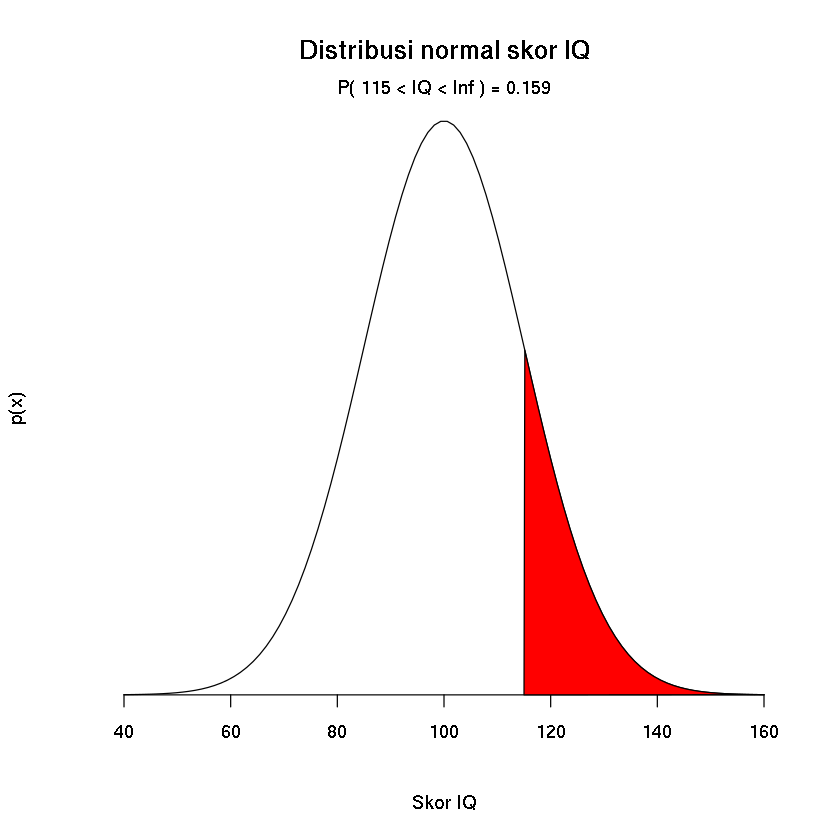
\includegraphics[width=0.9\textwidth]{gambar/gmb11.png}
    \caption{Distribusi normal IQ siswa.}
    \label{fig:fig11}
\end{figure}

\section{Laboratorium 5: Implementasi matriks kovarian di lingkungan R}
Kita akan membuat matriks kovarian di R dengan dua cara, yakni dengan membuat dari awal dan menggunakan fungsi bawaan (\textit{built-in}) dari R.

Mendefinisikan vektor kolom:


\begin{verbatim}
a <- 1:6
b <- seq(1, 11,by=2)
c <- seq(10, 60, by=10)
d <- c(2, 5, 5, 2, 1, 0)
e <- c(4, 5, 6, 7, 8, 9)        
\end{verbatim}



Membuat matriks dari vektor - vektor di atas:

\begin{verbatim}
M <- cbind(a,b,c,d,e)
k <- ncol(M)
n <- nrow(M)
print(M)        
\end{verbatim}

\begin{verbatim}
     a  b  c d e
[1,] 1  1 10 2 4
[2,] 2  3 20 5 5
[3,] 3  5 30 5 6
[4,] 4  7 40 2 7
[5,] 5  9 50 1 8
[6,] 6 11 60 0 9        
\end{verbatim}

Mencari rata - rata (ekspektasi) untuk setiap kolom:

\begin{verbatim}
k_rata2 <-  matrix(data = 1, nrow = n) %*% 
cbind(mean(a), mean(b), mean(c), mean(d), mean(e))
print(k_rata2)    
\end{verbatim}

\begin{verbatim}
     [,1] [,2] [,3] [,4] [,5]
[1,]  3.5    6   35  2.5  6.5
[2,]  3.5    6   35  2.5  6.5
[3,]  3.5    6   35  2.5  6.5
[4,]  3.5    6   35  2.5  6.5
[5,]  3.5    6   35  2.5  6.5
[6,]  3.5    6   35  2.5  6.5
\end{verbatim}


Mendefinisikan perbedaan antar matriks:

\begin{verbatim}
diffM <- M - k_rata2
print(diffM)
\end{verbatim}

\begin{verbatim}
        a  b   c    d    e
[1,] -2.5 -5 -25 -0.5 -2.5
[2,] -1.5 -3 -15  2.5 -1.5
[3,] -0.5 -1  -5  2.5 -0.5
[4,]  0.5  1   5 -0.5  0.5
[5,]  1.5  3  15 -1.5  1.5
[6,]  2.5  5  25 -2.5  2.5
\end{verbatim}

Mendefinisikan matriks kovarian:
\begin{verbatim}
Mkovar <- (n-1)^-1 * t(diffM) %*% 
diffM # kovarian sampel
print(Mkovar)
\end{verbatim}

\begin{verbatim}
     a  b   c     d    e
a  3.5  7  35  -2.5  3.5
b  7.0 14  70  -5.0  7.0
c 35.0 70 350 -25.0 35.0
d -2.5 -5 -25   4.3 -2.5
e  3.5  7  35  -2.5  3.5
\end{verbatim}

Mencari variansi dari matriks kovarian:
\begin{verbatim}
var <- diag(Mkovar)
print(var)
\end{verbatim}

\begin{verbatim}
    a     b     c     d     e 
  3.5  14.0 350.0   4.3   3.5 
\end{verbatim}

Kita dapat menggunakan fungsi \textit{built-in} \verb|cov()| untuk mendefinisikan matriks kovarian di lingkungan R:

\begin{verbatim}
print(cov(M))
\end{verbatim}

\begin{verbatim}
     a  b   c     d    e
a  3.5  7  35  -2.5  3.5
b  7.0 14  70  -5.0  7.0
c 35.0 70 350 -25.0 35.0
d -2.5 -5 -25   4.3 -2.5
e  3.5  7  35  -2.5  3.5
\end{verbatim}

\section{Distribusi - distribusi spesial}
Terdapat beberapa distribusi probabilitas yang umum dijumpai di hampir seluruh literatur tentang pemelajaran mesin, di antaranya adalah:
\subsection{Distribusi Bernoulli}
Merupakan suatu distribusi untuk peubah acak diskrit tunggal, dengan formulasi umum sebagai berikut:
\begin{equation}
    \begin{aligned}
        P(X=1) = \phi\\
        P(X=0) = 1 - \phi
    \end{aligned}    
\end{equation}
Distribusi ini dapat dikembangkan dengan melibatkan banyak peubah acak menjadi distribusi multinomial.

\subsection{Distribusi multinomial}
Distribusi yang melibatkan banyak peubah acak diskrit yang mana merupakan pengembangan dari distribusi Bernoulli. Kedua distribusi ini dapat dikatakan bisa memodelkan hampir seluruh distribusi probabilitas diskrit.

\subsection{Distribusi Gaussian}
Distribusi Gaussian (Gambar \ref{fig:fig12}) juga dikenal sebagai distribusi normal. Distribusi ini merupakan distribusi untuk peubah acak kontinyu yang dapat memodelkan hampir 90\% permasalahan statistik yang melibatkan bilangan riil. Oleh karenanya distribusi ini merupakan bagian integral dari hampir seluruh algoritma pemelajaran mesin yang melibatkan peubah acak kontinyu. Formulasi umum dari distribusi ini ditampilkan pada persamaan \ref{eqn:eqn49}:

\begin{equation}
    \mathcal{N}(x;\,\mu,\,\sigma^{2}) = \sqrt{\frac{1}{2\pi \sigma^2}} \exp{\left(-\frac{1}{2\sigma^2} (x-\mu)^2\right)}
    \label{eqn:eqn49}
\end{equation}

\begin{figure}[H]
    \centering
    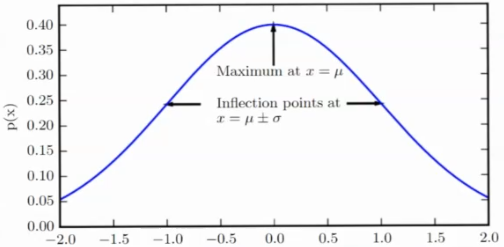
\includegraphics[width=0.9\textwidth]{gambar/gmb12.png}
    \caption{Distribusi normal.}
    \label{fig:fig12}
\end{figure}

Terdapat tiga buah aturan penting terkait sebaran data di dalam distribusi Gaussian, di antaranya adalah:
\begin{itemize}
    \item 68\% data tersebar di dalam jangkauan $\mu \pm{} \sigma$.
    \item 95\% data tersebar di dalam jangkauan $\mu \pm{} 2\sigma$.
    \item 99,7\% data tersebar di dalam jangkauan $\mu \pm{} 3\sigma$.
\end{itemize}

\subsection{Distribusi eksponensial}
Merupakan distribusi probabilitas kontinyu dengan titik lancip pada $x = 0$. Formulasi umumnya ditunjukkan pada persamaan \ref{eqn:eqn50} berikut ini:
\begin{equation}
    p(x;\,\lambda) = \lambda1_{x \geq 0} \exp{(-\lambda x)}
    \label{eqn:eqn50}
\end{equation}

\subsection{Distribusi Laplace}
Distribusi probabilitas dengan titik tajam pada $x = \mu$. $\mu$ di sini tidak harus berupa nilai rata - rata, melainkan titik sebarang tempat tempat titik lancip berada. Formulasi umumnya ditunjukkan pada persamaan \ref{eqn:eqn51} berikut ini:
\begin{equation}
      \text{Laplace}(x;\,\mu,\, \gamma) = \frac{1}{2\gamma}\exp{\left(\frac{-|x - \mu|}{\gamma}\right)}
      \label{eqn:eqn51}
\end{equation}

